\documentclass[10pt]{article} 
\usepackage{simpleConference}
\usepackage[utf8]{inputenc}
\usepackage{times}
\usepackage{graphicx}
\usepackage{amsmath, amsthm, amssymb}

% additional packages
\usepackage{tikz, tikz-3dplot} 
\usetikzlibrary{calc}
\usepackage{bbm}
\usepackage{support-caption}
\usepackage{subcaption}
\usetikzlibrary{matrix}
\usepackage{url}
\usepackage{float}

% macros
\newtheorem{prop}{Proposition}
\renewcommand{\vec}[1]{\mathbf{#1}}
\newcommand{\norm}[1]{\left\lVert#1\right\rVert}
\providecommand{\keywords}[1]{\textbf{\text{Keywords:}} #1}

\begin{document}

\title{A relationship between Likert-type responses and hypothetical latent variables\\
{\large Seminar for Computational Statistical Methods}}
\author{Marko Lalović \\
\\
November 2018 \\
}

\maketitle
\thispagestyle{empty}

\begin{abstract}
Researchers frequently collect responses to questionnaires in the Likert item format. A {\it Likert item} is a statement that the respondent is asked to evaluate by giving it a quantitative value on some dimension, with level of agreement being the dimension most commonly used. Here the {\it agreement} is defined as an underlying continuum that is unobserved and ranges from complete disagreement to complete agreement with the statement. Although researchers may be interested in responses for their own sake, they are often more interested in the analysis of the underlying agreement. Therefore the methods of analysis must involve a model for the relationship between Likert-type responses and the attitudes underlying them.

Accordingly, we introduce a model with which we remain in the context of the assumptions of the classical theory of the treatment of Likert-type responses. The response to a question is the observed {\it manifest variable}, denoted with $\hat{X}$, and we adopt the assumption that there exist a corresponding {\it latent variable}, denoted with $X$. Another assumption is that all questions are equivalent instruments for measuring the agreement.

We investigate the relationship between the variables $X$ and $\hat{X}$, particularly the optimal relationship in the ideal case. We derive a mapping from $X$ to $\hat{X}$, called {\it discretization}. Using optimal discretization and skew-normal distribution we show how we can simulate asymmetrically distributed Likert-type responses while maintaining the relationship between variables with nice mathematical properties. 

We also derive a mapping from $\hat{X}$ to $X$, called {\it reconstruction} that avoids arbitrary mapping of responses to numbers and the result allows the use of classical statistical methods. We investigate the simple problem of comparison of two means. We show that the common testing procedure is biased in general, since it doesn't take into account the discrete nature of Likert-type responses. Our proposed reconstruction procedure is based on the proportion of responses, as this provides minimal sufficient statistic for this problem. We illustrate our proposed testing procedure on a concrete example.
\end{abstract}

\keywords{Likert, Likert scale, Nonlinearity, Latent variable models, Statistical methodology}

\tableofcontents


\section{Introduction}
The diverse research community recognizes that the classical theory of analyzing the Likert-type responses requires improvement~\cite{Alphen}. The problems associated with the classical approach to analyzing Likert-type responses have already been discussed~\cite{Harwell}. Several alternative approaches have been proposed, even based on a methodology developed by quantum physicist~\cite{Camparo1}, \cite{Camparo2}. Our approach may be closer to item response theory~\cite{Jabrayilov}, \cite{Magno}, but we did not follow this theory and remained in the context of classical theory. Similar way of discretization to simulate Likert-type responses was used in~\cite{Boari}. They considered an additional condition and proposed a different algorithm that also allows for biased discretization. In the context of ordinal variables, optimal scaling using the nonlinear principal components method (NLPCA) is described in~\cite{Young} and~\cite{Gifi}. The introduction to NLPCA is found in~\cite{DeLeeuw}. We also do not assume a normal distribution of agreement in our model and instead model it as a skew-normal distribution similar to~\cite{Eijk}, which also includes a normal distribution. Rice, for example, stated~\cite{Rice} as early as 1938, that there is no obvious a priori reason for assuming a normal distribution when modeling agreement.

In Section~\ref{sec: model} we introduce a model where the distribution of agreement is described with a continuous random variable $X$ and the distribution of Likert-type responses with a discrete random variable $\hat{X}$. We are mainly trying to solve the following problem. We are interested in the relationship between the variables $X$ and $\hat{X}$. Our goal is to find the optimal mapping $\mathcal{D}$:
\begin{equation}
\mathcal{D}: X \rightarrow \hat{X}
\end{equation}
and the optimal mapping $\mathcal{R}$:
\begin{equation}
\mathcal{R}: \hat{X} \rightarrow X.
\end{equation}

This problem can also be described in the language of NLPCA as follows. Find the mappings $\mathcal{D}$ and $\mathcal{R}$ such that:
\begin{equation}
\hat{X} = \left( \mathcal{R} \circ \mathcal{D} \right) (X) + \epsilon,
\end{equation}
and minimize the expected value of the error $\norm{\epsilon^{2}}$. If we were to solve this problem using a neural network, we call such mappings {\it auto-associative neural network} or simply {\it autoencoder}. The optimal discretization is closely related to optimal scaling. Here we solve this problem using numerical methods, using the Lloyd-Max algorithm for optimal discretization and the adaptive Gauss-Newton method for optimal reconstruction. 

The mapping $\mathcal{D}$ is called {\it discretization}. We describe it in Section~\ref{sec: discretization} and show how we can use it to simulate Likert-type responses in Section~\ref{sec: simulation_likert}. The mapping $\mathcal{R}$ is called {\it reconstruction}. A procedure to reconstruct latent variables from Likert-type responses is in Section~\ref{sec: reconstruction}. In Section~\ref{sec: comparison-problem} we investigate the simple problem of comparison of two means in the context of our model. We first present a common approach, then we show it is biased in general. And finally illustrate our proposed testing procedure on a concrete example. We do not suggest using this approach in the case of small samples, as it fails on very small samples. In addition, we did not perform a theoretical analysis of the impact of sampling.

\section{Model} \label{sec: model}
The Likert-type response is the observed discrete random variable we call {\it manifest variable} and denote with $\hat{X}$. Suppose that there are more than two distinct possible responses: $K>2$, this means $\hat{X}$ is a {\it polytomous variable}. We denote the possible responses by $r_{k}$, $k = 1, ..., K$ and denote the probability that the value of $\hat{X}$ is $r_{k}$ with $p_{k}$. The distribution of the manifest variable $\hat{X}$ can be represented by the Table~\ref{tab: manifest}, where in the first row are the values $r_ {k}$ on which $\hat{X}$ is defined and in the second row are the probabilities $p_{k}$ that the value of $\hat{X}$ is $r_{k}$, for $k = 1, ..., K$.

\begin{table}[H]
\centering
\begin{tabular}{l|rrrrr}
  %\hline
	$r_{k}$ & $r_{1}$ & $r_{2}$ & ... & $r_{K-1}$ & $r_{K}$ \rule{0pt}{3ex} \\ 
  \hline
  	$\mathrm{P}(\hat{X} = r_{k})$ & $p_{1}$ & $p_{2}$ & ... & $p_{K-1}$ & $p_{K}$ \rule{0pt}{3ex} \\
   %\hline
\end{tabular}
\caption{ Distribution of a manifest variable $\hat{X}$.}
\label{tab: manifest}
\end{table}

We adopt the generally accepted assumption \cite{Bollen} that for each observed manifest variable $\hat{X}$ there exist a corresponding underlying continuum which lies in the minds of the subjects. We model this continuum with a continuous random variable we call {\it latent variable} and denote with $X$. Suppose the density of latent variable $X$ is defined on the set of real numbers and denote this density $f_{X}$. 

\begin{figure}[t]
	\centering
	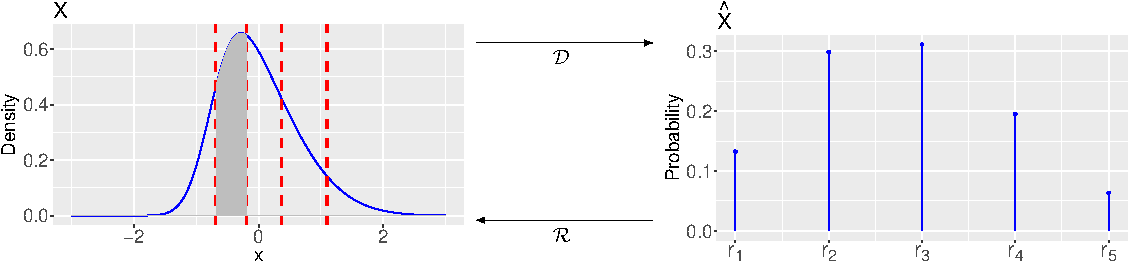
\includegraphics[width=\textwidth]{model.pdf}
	\caption{ Latent variable $X \sim \mathcal{SN}(-0.76, 1, 3)$ and the corresponding manifest variable $\hat{X}$.}
	\label{fig: model}
\end{figure}

Suppose the relation between $X$ and $\hat{X}$ is monotone and define the relation similarly to~\cite{Boari}:

\begin{equation} \label{eq: definicija}
\hat{X} = r_{k}, \qquad \text{if} \quad x_{k} < X \leq x_{k+1} \quad k = 1, ..., K+1,
\end{equation}
where the real numbers $x_{k}$ are called {\it thresholds}. The thresholds are defined in the domain of the corresponding latent variable $X$ and satisfy the constraints:
\begin{equation} \label{eq: constraints}
-\infty = x_{1} < x_{2} < ... < x_{K} < x_{K + 1} = \infty.
\end{equation}

For given thresholds $x_{k}$, $k = 1,...,K+1$ denote the intervals $\mathcal{R}_{k}$:  
\begin{equation}
\mathcal{R}_{1} = (-\infty, x_{2}], \quad ..., \quad \mathcal{R}_{k} = (x_{k}, x_{k+1}], \quad ..., \quad \mathcal{R}_{K} = (x_{K}, \infty)
\end{equation}
into which the thresholds $x_{k}$ partition the domain of the latent variable $X$.

The possible responses $r_{k}$ are called {\it representatives} of the intervals $\mathcal{R}_{k}$. The following relationship follows from the definition:
\begin{equation}
p_{k} = \mathrm{P}(\hat{X} = r_{k}) = f_{X}(x \in \mathcal{R}_{k}), \quad k = 1, ..., K. 
\end{equation}

We say that the random variable $\hat{X}$ is a {\it discretization} of the random variable $X$ and denote the mapping:
\begin{equation}
\mathcal{D}: X \rightarrow \hat{X}.
\end{equation}

We say that the random variable $X$ is a {\it reconstruction} of the random variable $\hat{X}$ and denote the mapping:
\begin{equation}
\mathcal{R}: \hat{X} \rightarrow X.
\end{equation}


\subsection{Sampling}
By sampling $X$ and then discretizing the sample, we get the same result as by discretizing $X$ and then sampling $\hat{X}$.

\begin{prop} \label{thm: sampling}
Denote by $\mathcal{S}$ the sampling from the random variable $X$ or $\hat{X}$. Denote by $\mathcal{D}$ the discretization of the continuous random variable $X$ or the sample $\vec{x}$ from the continuous random variable $X$. We claim that the diagram:

\begin{center}
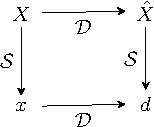
\includegraphics[width=0.17\textwidth]{diagram-cropped.pdf}
\end{center}

is commutative. Or in other words, this equation holds:
$$
\mathcal{D}(\mathcal{S}(X)) = \mathcal{S}(\mathcal{D}(X)).
$$
\end{prop}

\begin{proof}
Let $\vec{d} = \lbrace d_{i} \rbrace$ be the sample obtained by first sampling $X$ to obtain a sample $\vec{x} = \lbrace x_{i} \rbrace$ and then discretizing the sample $\vec{x}$ using thresholds $x_{k}$, $k \in \left\lbrace 1, ..., K+1 \right\rbrace$, as defined by Eq.~\ref{eq: definicija}. For $ k \in \left\lbrace 1, ..., K\right\rbrace$ it holds:
\begin{equation}
r_{k} \in d, \qquad \text{if there exists} \quad x_{i} \in \vec{x}, \quad \text{such that} \quad x_{k} < x_{i} \leq x_{k + 1}
\end{equation}

Or in other words, let
$$
\vec{d} = \mathcal{D}(\mathcal{S}(X)).
$$

The probability that $r_{k}$ is in sample $\vec{d}$ is 
$$
\mathrm{P}(x_{k} < X \leq x_{k+1})
$$
which is exactly $p_{k}$ in the definition of $\hat{X} = \mathcal{D}(X)$.
\end{proof}

Let us also determine the distribution of the sample $\vec{d}$ of size $n$. Denote by $b_{k}$ the number of responses with the value $r_{k}$ in the sample $\vec{d}$. The sample $\vec{d}$ has a multinomial distribution:
\begin{equation} \label{eq: sampling}
\mathrm{P}(\lbrace b_{k} \mid k = 1,...,K \rbrace) = \binom{n}{b_{1}, ..., b_{K}} \prod_{k = 1}^{K} p_{k}^{b_{k}},
\end{equation}
for $b_{k} \in \lbrace 0, ..., n \rbrace$ and where $\sum_{k=1}^{K}{b_{k}} = n$.

\subsection{Skew normal distribution}
We model the latent variable $X$, similar to~\cite{Eijk}, by skew-normal distribution $\mathcal{SN}(\xi, \omega, \alpha)$. Where $\xi$ is the location parameter, $\omega$ is the scaling parameter, and $\alpha$ is asymmetry parameter. We present the skew-normal distribution in more detail.

The random variable $X$ has a {\it standard skew-normal distribution}~\cite{Azzalini} with parameter $\alpha$, if it's probability density function is:

\begin{equation}
f(x, \alpha) = 2 \cdot \phi(x) \cdot \Phi(\alpha x),
\end{equation}

where $\alpha$ and $x$ are real numbers, $\phi(\cdot)$ density, and $\Phi(\cdot)$ cumulative distribution function of the standard normal distribution. Denote by $X \sim \mathcal{SN}(\alpha)$. It is easy to check:
\begin{itemize}
	\item When $\alpha = 0$ asymmetry disappears and we get the density of the normal distribution.
	\item The distribution is left asymmetric when $\alpha > 0$ and right asymmetric when $\alpha < 0$.
	\item As $|\alpha|$ increases, the asymmetry increases and converges to the so-called {\it half normal density}.
\end{itemize}

Let $X \sim \mathcal{SN}(\alpha)$ and use the linear transformation $Y = \omega X + \xi$, where $\xi$ is called the {\it location parameter} and $\omega$ {\it scaling parameter}. Then $Y$ is distributed {\it skew-normal} with density:

\begin{equation}
f_{Y}(y; \xi, \omega, \alpha) = \frac{2}{\omega} \cdot
\phi\left(\frac{y - \xi}{\omega}\right) \cdot
\Phi\left(\alpha \left( \frac{y - \xi}{\omega} \right)\right),
\end{equation}
where $\xi$ is a real number and $\omega$ is a positive real number. Denote by $Y \sim \mathcal{SN}(\xi, \omega, \alpha)$. \\

We assume the latent variable has a skew-normal distribution:
\begin{equation}
X \sim \mathcal{SN}(\xi, \omega, \alpha)
\end{equation}
for some parameter values $\xi$, $\omega$ and $\alpha$.

In Figure~\ref{fig: model} there is an example of the latent variable $X \sim \mathcal{SN}(-0.76, 1, 3)$ and the corresponding manifest random variable $\hat{X}$ for $K = 5$. The thresholds $x_{k}$, $k = 2, ..., 5$ are drawn in dashes and the shaded area equals to the probability:

$$
p_{2} = \mathrm{P}(\hat{X} = r_{2}) = f_{X}(x \in \mathcal{R}_{2}).
$$

\section{Discretization} \label{sec: discretization}
In general the discretization problem can be described as follows. For a given $K$, we wish to find a tessellation, which determines the partition of the continuous continuum of the domain of the continuous random variable $X$ into $K$ subsets on which we can define a probability distribution and obtain a discrete random variable $\hat{X}$ defined on some set $r_{k}$, $k = 1, ..., K$. In our case, where the domain of $X$ is one-dimensional set of real numbers, we wish to find the thresholds:
$$
x_{k}, \quad k = 1, ..., K + 1,
$$
which divide the interval on which $X$ is defined into $K$ subintervals $\mathcal{R}_{k}$, on which we can define the probability distribution. At the same time, we require that the thresholds satisfy the Condition~\ref{eq: constraints}, so we can already set the edge thresholds to:
$$
x_{1} = -\infty, x_{K + 1} = \infty.
$$

\subsection{Equal width discretization} \label{sec: EW}
One of the most commonly used~\cite{Wu} techniques of discretization is the use of equally wide intervals, the so-called ‘Equal Width Interval Binning’ (EW) discretization. The reason why this method is so popular is probably that it is easy to understand and the implementation is trivial.

\paragraph{Description of the equal width discretization procedure.} In the case where we have a continuous random variable $X$ defined on an unbounded interval, we have to select a subinterval on which the majority of the density $f_{X}$ is defined. The popular choice is the interval $[a, b]$ for the random variable $X$, where the boundaries are: 
\begin{align*}
a &= \mathrm{E}[X] - 3 \cdot \mathrm{sd}(X), \\
b &= \mathrm{E}[X] + 3 \cdot \mathrm{sd}(X).
\end{align*}

In the case of $X \sim N(0, 1)$, the interval is $[-3, 3]$. Then we divide the interval $[a, b]$ into $K$ equally wide intervals with thresholds:
$$
\quad x_{2}, \quad x_{3}, \quad ..., \quad x_{K},
$$
which define the middle thresholds of EW discretization. The result we get with the described procedure satisfies the Condition~\ref{eq: constraints} and we have a necessary and sufficient condition for the probability distribution on some set of responses $r_{k}$, $k = 1, .., K$.

\subsection{Optimal discretization}
Let us find the optimal thresholds $x_{k}$ and optimal representatives $r_{k}$, so that the discretization $\hat{X}$ will be the best approximation of $X$ by some criterion. 

For this purpose, define the function $q: \mathbb{R} \rightarrow \mathbb{R}$:

\begin{equation}
q(x) = r_{k}, \quad \text{if} \quad x \in \mathcal{R}_{k},
\end{equation}

which assigns to each $x \in \mathbb{R}$ a representative $r_{k}$. The function $q$ is called {\it quantization}~\cite{Gonzalez}. The function $q$ is defined with $K-1$ by thresholds $x_{2}, ..., x_{K}$ and $K$ representatives $r_{1}, ..., r_{K}$.

\paragraph{Description of the optimal discretization procedure.}
For a given $K$, we need to find the thresholds $x_{k}$ and representatives $r_{k}$ of the intervals $\mathcal{R}_{k}$ such that they minimize the mean square error (MSE):
\begin{align} \label{eq: eps}
\epsilon &= \int_{-\infty}^{\infty} \left( x - q(x) \right)^{2} \cdot f_{X}(x) dx \\
&= \sum_{k = 1}^{K} \int_{x_{k}}^{x_{k+1}} \left( x - r_{k} \right)^{2} \cdot f_{X}(x) dx.
\end{align}

To find the minimum of $\epsilon$ with respect to $x_{k}$ and $r_{k}$ we set the equations:
\begin{align}
\frac{\partial \epsilon}{\partial x_{k}} &= 0
\implies (x_{k} - r_{k-1})^{2} \cdot f_{X}(x_{k}) - 
(x_{k} - r_{k})^{2} \cdot f_{X}(x_{k}) = 0 \label{eq: part_xk} \\
\frac{\partial \epsilon}{\partial r_{k}} &= 0
\implies 2 \cdot \int_{x_{k}}^{x_{k+1}} (x - r_{k}) \cdot f_{X}(x)dx = 0, \quad k = 1,...,K. \label{eq: part_rk}
\end{align}

From the obtained equations we express $x_{k}$ and $r_{k}$ to derive the conditions:
\begin{align} 
x_{k} &= \frac{r_{k-1} + r_{k}}{2}, \quad k = 2, ..., K \label{eq: xk} \\
r_{k} &= \frac{ \int_{x_{k}}^{x_{k+1}} x \cdot f_{X}(x) dx }{ \int_{x_{k}}^{x_{k+1}} f_{X}(x) dx }, \quad k = 1,...,K. \label{eq: rk}
\end{align}

We can also check the sufficiency of the derived conditions. If all the second order partial derivatives~\ref{eq: part_xk} and \ref{eq: part_rk} with respect to $x_{k}$ and $r_{k}$ exist, then the critical point determined by the Conditions~\ref{eq: xk} and \ref{eq: rk} is really the minimum, if the matrix of second order  partial derivatives is positive definite.

Let's interpret the result. Optimal thresholds $x_{k}$ lie between the optimal representatives $r_{k}$ and optimal representatives $r_{k}$ are centroids of the density $f_{X}$ between the successive thresholds $x_{k}$. This resulting tessellation of $X$ is called {\it weighted centroid Voronoi tessellation}, because it is weighted with respect to the density $f_{X}$ and centroid, because the representative of each cell is the centroid of that cell. 


For optimal discretization we can use the Lloyd-Max~\cite{Max} algorithm. This algorithm is very similar to the k-means algorithm, it repeatedly finds the centroid of each set and then rearranges the boundaries of the sets, but the input to the algorithm is a continuous rather than a discrete set. In our examples when using skew-normal distribution, the convergence is fast and we stop after 10 iterations. 

We can imagine the optimal discretization as an orthogonal projection $\mathcal{D}$ of a continuous random variable $X$ from latent space to manifest space:

\begin{center}
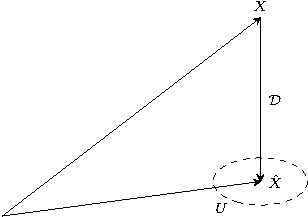
\includegraphics[width=0.4\textwidth]{projection-cropped.pdf}
\end{center}

When using Lloyd-Max algorithm we allow some error. Thus, the resulting discretization is a discrete random variable $\hat{X}$ from the neighborhood $U$ of the orthogonal projection $\mathcal{D}$ of $X$ from latent space to manifest space.

\subsection{Properties of optimal discretization}
We list some important properties of the optimal discretization $\hat{X}$ of a continuous random variable $X$.

\begin{prop} \label{thm: E}
Optimal discretization is unbiased:
\begin{equation}
\mathrm{E}[X] = \mathrm{E}[\hat{X}]
\end{equation}
\end{prop}

\begin{proof}
It follows from the Condition~\ref{eq: rk} for $r_{k}$:
\begin{align*}
\mathrm{E}[\hat{X}] &= \sum_{k=1}^{K} r_{k} \int_{x_{k}}^{x_{k+1}} f_{X}(x) dx \\
	&= \sum_{k=1}^{K} \int_{x_{k}}^{x_{k+1}} x \cdot f_{X}(x) dx \\
	&= \int_{x_{1}}^{x_{K+1}} x \cdot f_{X}(x) dx \\
	&= \mathrm{E}[X].
\end{align*}
\end{proof}



\begin{prop} \label{thm: decor}
The error we make with optimal discretization is orthogonal or decorrelated with a random variable $\hat{X}$:
\begin{equation}
\mathrm{E} \left[ \left(X - \hat{X}\right) \cdot \hat{X} \right] = 0.
\end{equation}
\end{prop}

\begin{proof}
Equivalently we must show
$$
\mathrm{E}[X \cdot \hat{X}] = \mathrm{E}[\hat{X}^{2}].
$$
Formally $\hat{X}$ must be treated as a continuous random variable with density $f_{\hat{X}}$, which is a step function defined on the set of real numbers:
\begin{equation}
f_{\hat{X}}(\hat{x}) = \sum_{k = 1}^{K} p_{k} \cdot \mathbbm{1}_{\mathcal{R}_{k}}(\hat{x}), \quad \hat{x} \in \mathbb{R}
\end{equation}
where $\mathbbm{1}_{\mathcal{R}_{k}}$ is an indicator function:
\[ \mathbbm{1}_{\mathcal{R}_{k}}(\hat{x}) =  \left\{
\begin{array}{ll}
      1, & \text{if} \quad \hat{x} \in  \mathcal{R}_{k}\\
      0, & \text{if} \quad \hat{x} \not\in  \mathcal{R}_{k}.\\      
\end{array}
\right. \]
Correlation between $X$ and $\hat{X}$ is then:
$$
\mathrm{E}[X \cdot \hat{X}] = \sum_{k=1}^{K} \int_{x_{k}}^{x_{k+1}} 
x \cdot \hat{x} \cdot
f_{X, \hat{X}} (x, \hat{x} = r_{k}) dx.
$$

When $x \in \mathcal{R}_{k}$, the total density can be written as
$$
f_{\hat{X}}(\hat{x} = r_{k} \mid \hat{x} \in \mathcal{R}_{k} ) \cdot
f_{X}( x \in \mathcal{R}_{k} ) = f_{X}(x \in \mathcal{R}_{k}).
$$
That is why
$$
\mathrm{E}[X \cdot \hat{X}] = \sum_{k=1}^{K} r_{k} \int_{x_{k}}^{x_{k+1}} 
x \cdot f_{X} (x) dx.
$$

From Condition~\ref{eq: rk} and Proposition~\ref{thm: E} follows:
\begin{align*}
\mathrm{E}[X \cdot \hat{X}] &= \sum_{k=1}^{K} r_{k} \int_{x_{k}}^{x_{k+1}} 
x \cdot f_{X} (x) dx \\ 
&= \sum_{k=1}^{K} r_{k}^{2} \cdot f_{\hat{X}} (\hat{x} = r_{k}) \\
&= \mathrm{E}[\hat{X}^{2}].
\end{align*}
\end{proof}

The consequence of the Propositions~\ref{thm: E} and \ref{thm: decor} is as follows. 
\begin{prop} \label{thm: var_diff}
Variance of optimal discretization $\hat{X}$ is:
\begin{equation}
\mathrm{var}(\hat{X}) = \mathrm{var(X)} + \epsilon,
\end{equation}
where $\epsilon \in \mathbb{R}$ is minimal for a given random variable $X$.
\end{prop}

\begin{proof}
Similar to the proof of Proposition~\ref{thm: decor}, we must treat $\hat{X}$ as a continuous random variable. Using Propositions~\ref{thm: E}, \ref{thm: decor}:
\begin{align*}
\epsilon &= \mathrm{E}[ \left( X - \hat{X} \right)^{2} ] \\
&= \mathrm{E}[X^{2} - 2\cdot X \cdot \hat{X} + \hat{X}^{2}] \\
&= \mathrm{E}[X^{2}] - 2 \cdot \mathrm{E}[\hat{X}^{2}] + \mathrm{E}[\hat{X}^{2}] \\ 
&= \mathrm{E}[X^{2}] - \mathrm{E}[\hat{X}^{2}] \\ 
&= \left( \mathrm{E}[X^{2}] - \mathrm{E}[X]^{2} \right) - 
\left( \mathrm{E}[\hat{X}^{2}] - \mathrm{E}[\hat{X}]^{2} \right) \\
&= \mathrm{var}(X) - \mathrm{var}(\hat{X}).
\end{align*}
\end{proof}


\section{Simulation of Likert-type responses} \label{sec: simulation_likert}

\subsection{Common approach}

One of the most commonly used~\cite{Wu} approaches of simulating Likert-type item responses is to choose a normal distribution with some mean and variance for the underlying latent variable $X$. And then sample from this distribution to get a random sample $\vec{x}$. Then discretize $\vec{x}$ using using equal width discretization to simulate a random sample $\hat{\vec{x}}$ from manifest variable $\hat{X}$.

To simulate responses that are distributed asymmetrically can be achieved by adjusting the widths of the intervals of EW discretization. For example for the right asymmetry, we can set each interval to be half as narrow as the previous one. 

The problem with this approach is the lack of control. There are no guarantees of what the result would be. If we do not take into account the relationship between $X$ and $\hat{X}$, then evaluating the statistical methods with such a simulation process can be questionable at least.

\subsection{Proposed approach}

\begin{figure}[t]
	\centering
	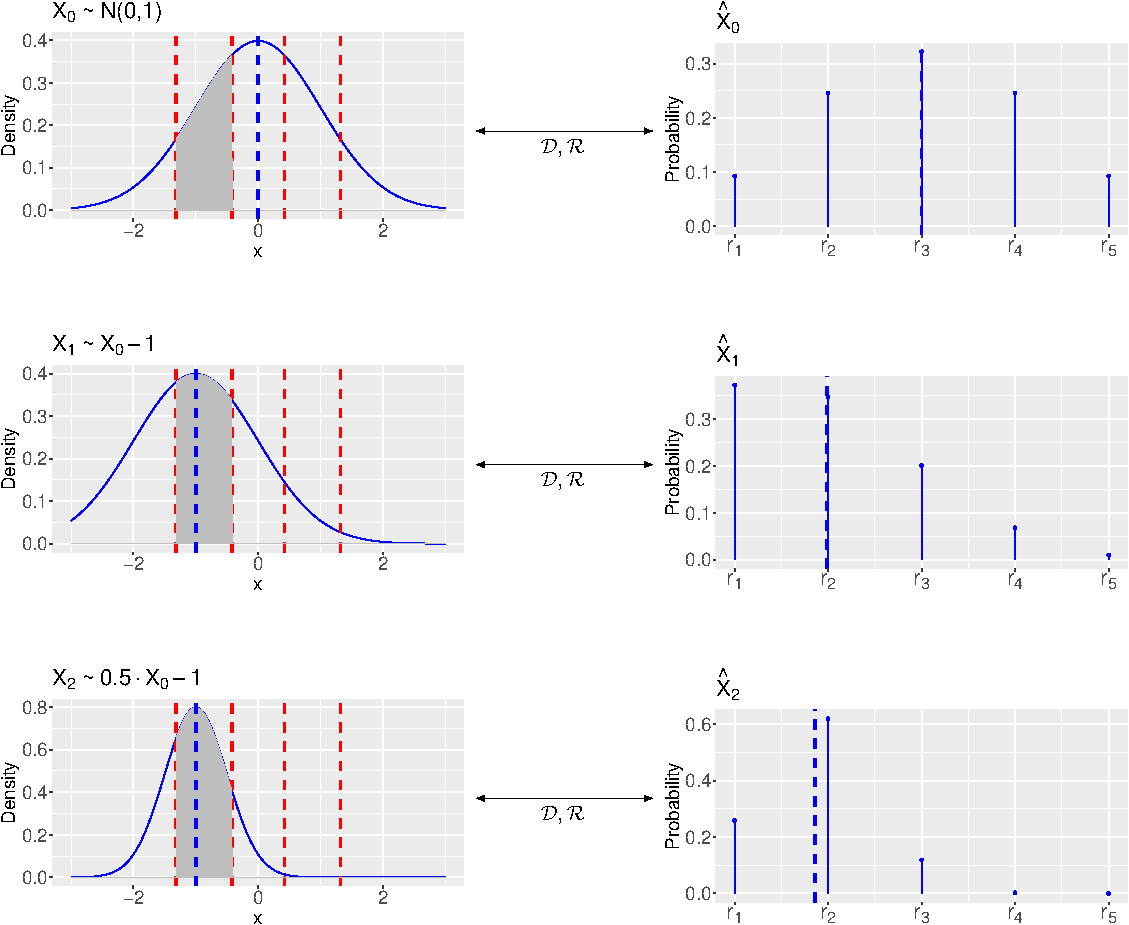
\includegraphics[width=\textwidth]{problem-cropped.pdf}
	\caption{ Examples of pairs $X_{i}$, $\hat{X}_{i}$.}
	\label{fig: problem-definition}
\end{figure}

Let there be $K$ possible responses $r_{k}$, $k = 1,...,K$, which measure say people's agreement with some abstract idea. Imagine a hypothetical population of people with an underlying latent variable $X_{0}$ with expected value:
\begin{equation}
\mathrm{E}[X_{0}] = 0
\end{equation}
and variance:
\begin{equation}
\mathrm{var}(X_{0}) = \sigma^{2}.
\end{equation}
We call this population {\it neutral}, because we can say they are on average neutral about this abstract idea. Let $\hat{X}_{0}$ be the manifest variable, obtained by using the thresholds $x_{k}$ and defined on responses $r_{k}$. The probability that $\hat{X}_{0}$ equals $r_{k}$ is by definition:
\begin{equation}
\mathrm{P}(\hat{X}_{0} = r_{k}) = f_{X}(x \in \mathcal{R}_{k}), \quad k = 1, ..., K.
\end{equation}

The expected value of the manifest variable is then:
\begin{equation}
\mathrm{E}[\hat{X}_{0}] = 0
\end{equation}
and variance is:
\begin{equation}
\mathrm{var}(\hat{X}_{0}) = \mathrm{var}(X_{0}) + \epsilon,
\end{equation}
where $\epsilon \in \mathbb{R}$ is minimal for a given latent variable $X_{0}$ when the manifest variable is the optimal discretization of $X_{0}$. That is when the responses $r_{k}$ are the optimal representatives of the intervals $\mathcal{R}_{k}$. 

Imagine some other hypothetical population with underlying latent variable $X_{i}$:
\begin{equation}
X_{i} \sim \omega_{i} \cdot X_{0} + \xi_{i}
\end{equation}
for some real number $\xi_{i}$ and for some positive real number $\omega_{i}$. For example, for $\xi_{i} < 0$, this population on average agrees for $\xi_{i}$ less with this abstract idea than neutral population, and for $\omega_{i} < 1$, the agreement of this population is less dispersed than in neutral population. The same responses $r_{k}$, $k = 1,...,K$ are available to this population. Therefore the probability that $\hat{X}_{i}$ is $r_{k}$ equals:
\begin{equation}
\mathrm{P}(\hat{X}_{i} = r_{k}) = f_{X_{i}}(x \in \mathcal{R}_{k}), \quad k = 1, ..., K.
\end{equation}

Examples of pairs: $X_{i}$, $\hat{X}_{i}$ for $i=0,1,2$ are in Figure~\ref{fig: problem-definition}, where $X_{0} \sim N(0,1)$, $\xi_{1} = \xi_{2} = -1$, $\omega_{1}=1$ and $\omega_{2}=0.5$. In the Figure, the density $f_{X_{i}}$ and the distribution $\hat{X}_{i}$ is shown in blue, the thresholds $x_{k}$, $k = 2, ..., 5$ dashed in red, area $p_{2} = \mathrm{P}(\hat{X}_{i} = 2)$ with grey, and the expected values are dashed in blue.

To simulate asymmetric manifest variables, we can choose $X_{0} \sim \mathcal{SN}(\alpha)$, for some $\alpha \neq 0$. 

This simulation approach can be very useful for having more control, as the relationship between pairs $X_{i}$, $\hat{X}_{i}$ is preserved, as we did not use biased discretization.


\section{A procedure to reconstruct latent variables} \label{sec: reconstruction}

Optimal estimator of $p_{k}$ for the manifest random variable $\hat{X}$ of some population is:
\begin{equation}
\hat{p}_{k} = \frac{b_{k}}{n},
\end{equation}
where $b_{k}$ is the number of responses with the value $r_{k}$ and $n$ is the number of all responses. This follows from Eq.~\ref{eq: sampling}.
In this reconstruction procedure we assume optimal thresholds. Responses $r_{k}$ are arbitrary, they can be: totally disagree, ...., completely agree.

Based on the sample from $\hat{X}$, we would like to find the values of parameters $\alpha$, $\xi$, $\omega$ and thus reconstruct the latent variable, which we assume follows the skew-normal distribution:
\begin{equation}
X \sim \omega \cdot X_{0}(\alpha) + \xi
\end{equation}
Let the random variable $X_{0}$ be the latent variable of the neutral population:
\begin{equation}
X_{0}(\alpha) \sim X - \mu
\end{equation}
where $X \sim \mathcal{SN}(\alpha)$ and $\mu = \mathrm{E}(X)$. The parameters $\alpha, \xi, \omega$ describe the whole family of skew-normal distributed random variables. We see that $\hat{X}$ is well defined because we have assumed the thresholds $x_{k}(\alpha)$ which discretize $X_{0}(\alpha)$ for each value of $\alpha$.

\subsection{Estimation of parameters $\xi$ and $\omega$} 
For a given $\alpha = \alpha_{0}$:
\begin{align}
p_{k} &= 
F_{\omega \cdot (X - \mu) + \xi}(x_{k+1}) -
F_{\omega \cdot (X - \mu) + \xi}(x_{k}) \\
&= F_{X}(\frac{x_{k+1} - \xi}{\omega} + \mu) -
F_{X}(\frac{x_{k} - \xi}{\omega} + \mu), \qquad k = 1, ..., K.
\end{align}

From this we obtain an overdetermined system of $K$ nonlinear equations for parameters $\xi$ and $\omega$:
\begin{equation}
g_{k}(\xi, \omega) = 
F_{X}(\frac{x_{k+1} - \xi}{\omega} + \mu) -
F_{X}(\frac{x_{k} - \xi}{\omega} + \mu) - p_{k}, \qquad k = 1, ..., K.
\end{equation}

This is a nonlinear least squares problem that can only be solved numerically because $F_{X}$ is not expressed by elementary functions. For greater stability, we reparametrize it:
\begin{align}
u &= \xi \\
v &= 1/\omega,
\end{align}

and obtain a new system of equations:
\begin{equation}
h_{k}(u, v) = 
F_{X}(v \cdot x_{k+1} - v \cdot u + \mu) -
F_{X}(v \cdot x_{k} - v \cdot u + \mu) - p_{k}, \qquad k = 1, ..., K,
\end{equation}

which can be written in matrix form:
\[ H(u,v) = \left( \begin{array}{cc}
h_{1}(u,v) \\
. \\
. \\
. \\
h_{K}(u,v) \\ \end{array} \right).
\]

And compute partial derivatives:
\begin{align*}
\frac{\partial h_{k}}{\partial u} &= f_{X}(v \cdot x_{k+1} - v \cdot u + \mu) \cdot (-v) - f_{X}(v \cdot x_{k} - v \cdot u + \mu) \cdot (-v) \\
\frac{\partial h_{k}}{\partial v} &= f_{X}(v \cdot x_{k+1} - v \cdot u + \mu) \cdot (x_{k+1} - u) 
- f_{X}(v \cdot x_{k} - v \cdot u + \mu) \cdot (x_{k} - u)
\end{align*}

For the edge cases where $x_{1} = -\infty$ or $x_{K} = \infty$, the limit $f_{X}(x)$, when $x$ goes to $-\infty$ or $\infty$, equals to 0 and the terms with $x_{1}$ and $x_{K}$ can be omitted. We obtain the Jacobian matrix:
\[ J(u,v) = \left( \begin{array}{ccc}
\frac{\partial h_{1}}{\partial u} & \frac{\partial h_{1}}{\partial v} \\
. & . \\
. & . \\
\frac{\partial h_{K}}{\partial u} & \frac{\partial h_{K}}{\partial v} \\ \end{array} \right) \mid (u,v)
\]
and solve the system using the Gauss-Newton method, starting from an initial guess: 
$$
(u_{0}, v_{0}) = (0, 1)
$$ 

and finding $(u_{*}, v_{*})$ which minimizes the second norm:
\begin{equation}
\norm{H(u_{*}, v_{*})}_{2}.
\end{equation}


The Gauss-Newton method was implemented as follows. At each step, we evaluate the Jacobian matrix
$$
A = J(u_{i}, v_{i})
$$

and decompose into singular values: 
$$
A = U D V.
$$

The correction $d$ for $(u_{i}, v_{i})$ is calculated by solving the linear least squares problem, obtaining:
$$
d = V' D^{-1} U' H(u_{i}, v_{i}).
$$

and finding the next approximation:
$$
(u_{i+1}, v_{i+1}) = (u_{i}, v_{i}) + d_{*}.
$$

Implementation is adaptive in the following way. We adjust the correction $d$ at each step $i$ as needed. While the value of correction $d$ yields:
$v_{i+1} < 0,$
we halve the correction $d$:
$$
d := d/2.
$$
This way we reduce the value $d$ exponentially, until we get the first appropriate value of correction $d$. The value of $v_{i}$ must not be less than 0, because $\omega > 0$. 

An example is in Figure~\ref{fig: newton_trace}, which shows a trace of approximations obtained by the adaptive Gauss-Newton method when reconstructing the parameters:
\begin{align*}
\xi &= 0.2 \cdot \mathrm{sd}(X) \approx 0.123 \\
\omega &= 0.5
\end{align*}
and $X \sim \mathcal{SN}(\alpha)$ where $\alpha = 6.3$. In this case $v = 2$ and $u = \xi$. 

\begin{figure}
  \centering
  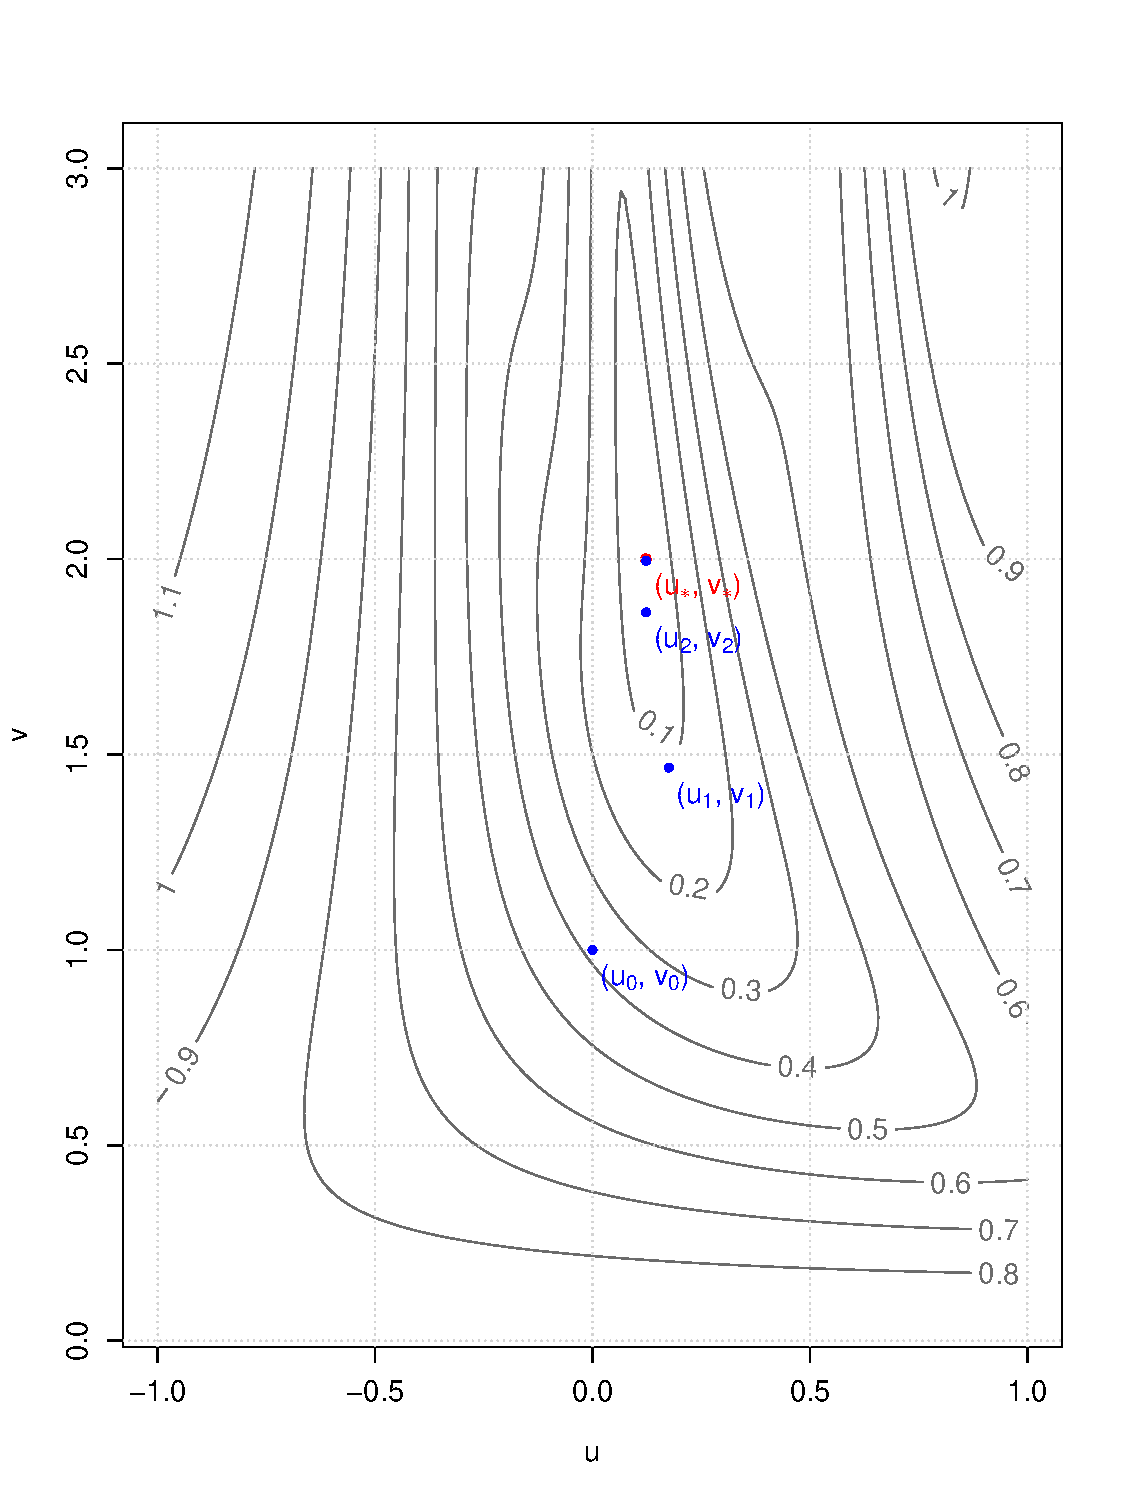
\includegraphics[width=0.4\linewidth]{newton_trace_WCVT.pdf}
  \caption{ Trace of approximations using the adaptive Gauss-Newton method.}
  \label{fig: newton_trace}
\end{figure}


\subsection{Estimation of parameter $\alpha$} 

The sample from asymmetric manifest variable $\hat{X}$ may look symmetric ($\alpha = 0$) when in fact comes from an asymmetric distribution ($\alpha \neq 0$). Therefore, the value of $\alpha$ is estimated as follows.

For each value $\alpha_{i}$ of parameter $\alpha$ we calculate the corresponding values of $\xi_{i}$ and $\omega_{i}$ using the procedure already described. This procedure reconstructs some continuous random variable $X_{i}$. We discretize it using thresholds $x_{k}(\alpha_{i})$ to get $\hat{X}_{i}$, which has probabilities $\hat{p}_{i}$.

If the value $\alpha_{i}$ of parameter $\alpha$ is far from the actual value, then $\hat{p}_{k}$ are far from the actual $p_{k}$. We can calculate the error: 
\begin{equation}
\epsilon = \sum_{k=1}^{K} (\hat{p}_{k} - p_{k})^{2}.
\end{equation}

We choose the value of $\alpha$, which minimizes the error $\epsilon$. 

\begin{figure}[H]
\centering
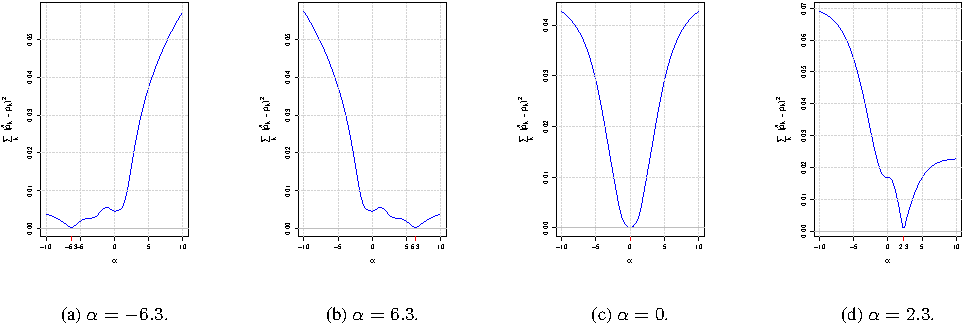
\includegraphics[width=\linewidth]{parameter-alpha-cropped.pdf}
\caption{ Estimation of the value of parameter $\alpha$.}
\label{fig: alpha_reconstruction}
\end{figure}

Examples of reconstructions are in Figure~\ref{fig: alpha_reconstruction} for different actual parameter values. For example, if the actual value of $\alpha$ is negative, the error $\epsilon$ in terms of the value of $\alpha$ is shown in Figure~\ref{fig: alpha_negative}. The actual values of parameters $\xi$ and $\omega$ only affect the shape of the function of error $\epsilon$ in terms of $\alpha$ and do not effect at which value of $\alpha$ the minimum error $\epsilon$ is reached.

\subsection{Estimation of parameters from a sample}
As the value of $|\alpha|$ increases, the density of the random variable $X \sim \mathcal{SN}(\alpha, \cdot, \cdot)$ converges to half normal density. For values $|\alpha|$ greater than 10, the differences between the distributions are negligible. Therefore, we limit ourselves to the interval $[-10, 10]$ on which we look for the value of $\alpha$ and choose a denser division near $\alpha = 0$, where the differences between the distribution are greatest. From a small sample sizes, we can get estimates that are very different from the actual values of parameters. However, for larger sample sizes, the estimates are very close to the true values. For example, for the sample size $n=1000$ and actual parameters:

\begin{align*}
\alpha &= 0 \\
\xi &= -1 \\
\omega &= 1
\end{align*}

we get estimates:
\begin{align*}
\alpha &= -0.2000000 \\
\xi &= -0.9893231 \\
\omega &=  1.0012696
\end{align*}

The reconstruction is shown in Figure~\ref{fig: reconstruction_on_sample}. 
On small sample sizes the shape of the error function $\epsilon$ in terms of $\alpha$ can even become concave. We select the value of $\alpha$, where the first select the value of the alpha parameter where extreme value of error function $\epsilon$ is reached.

\begin{figure}
\centering
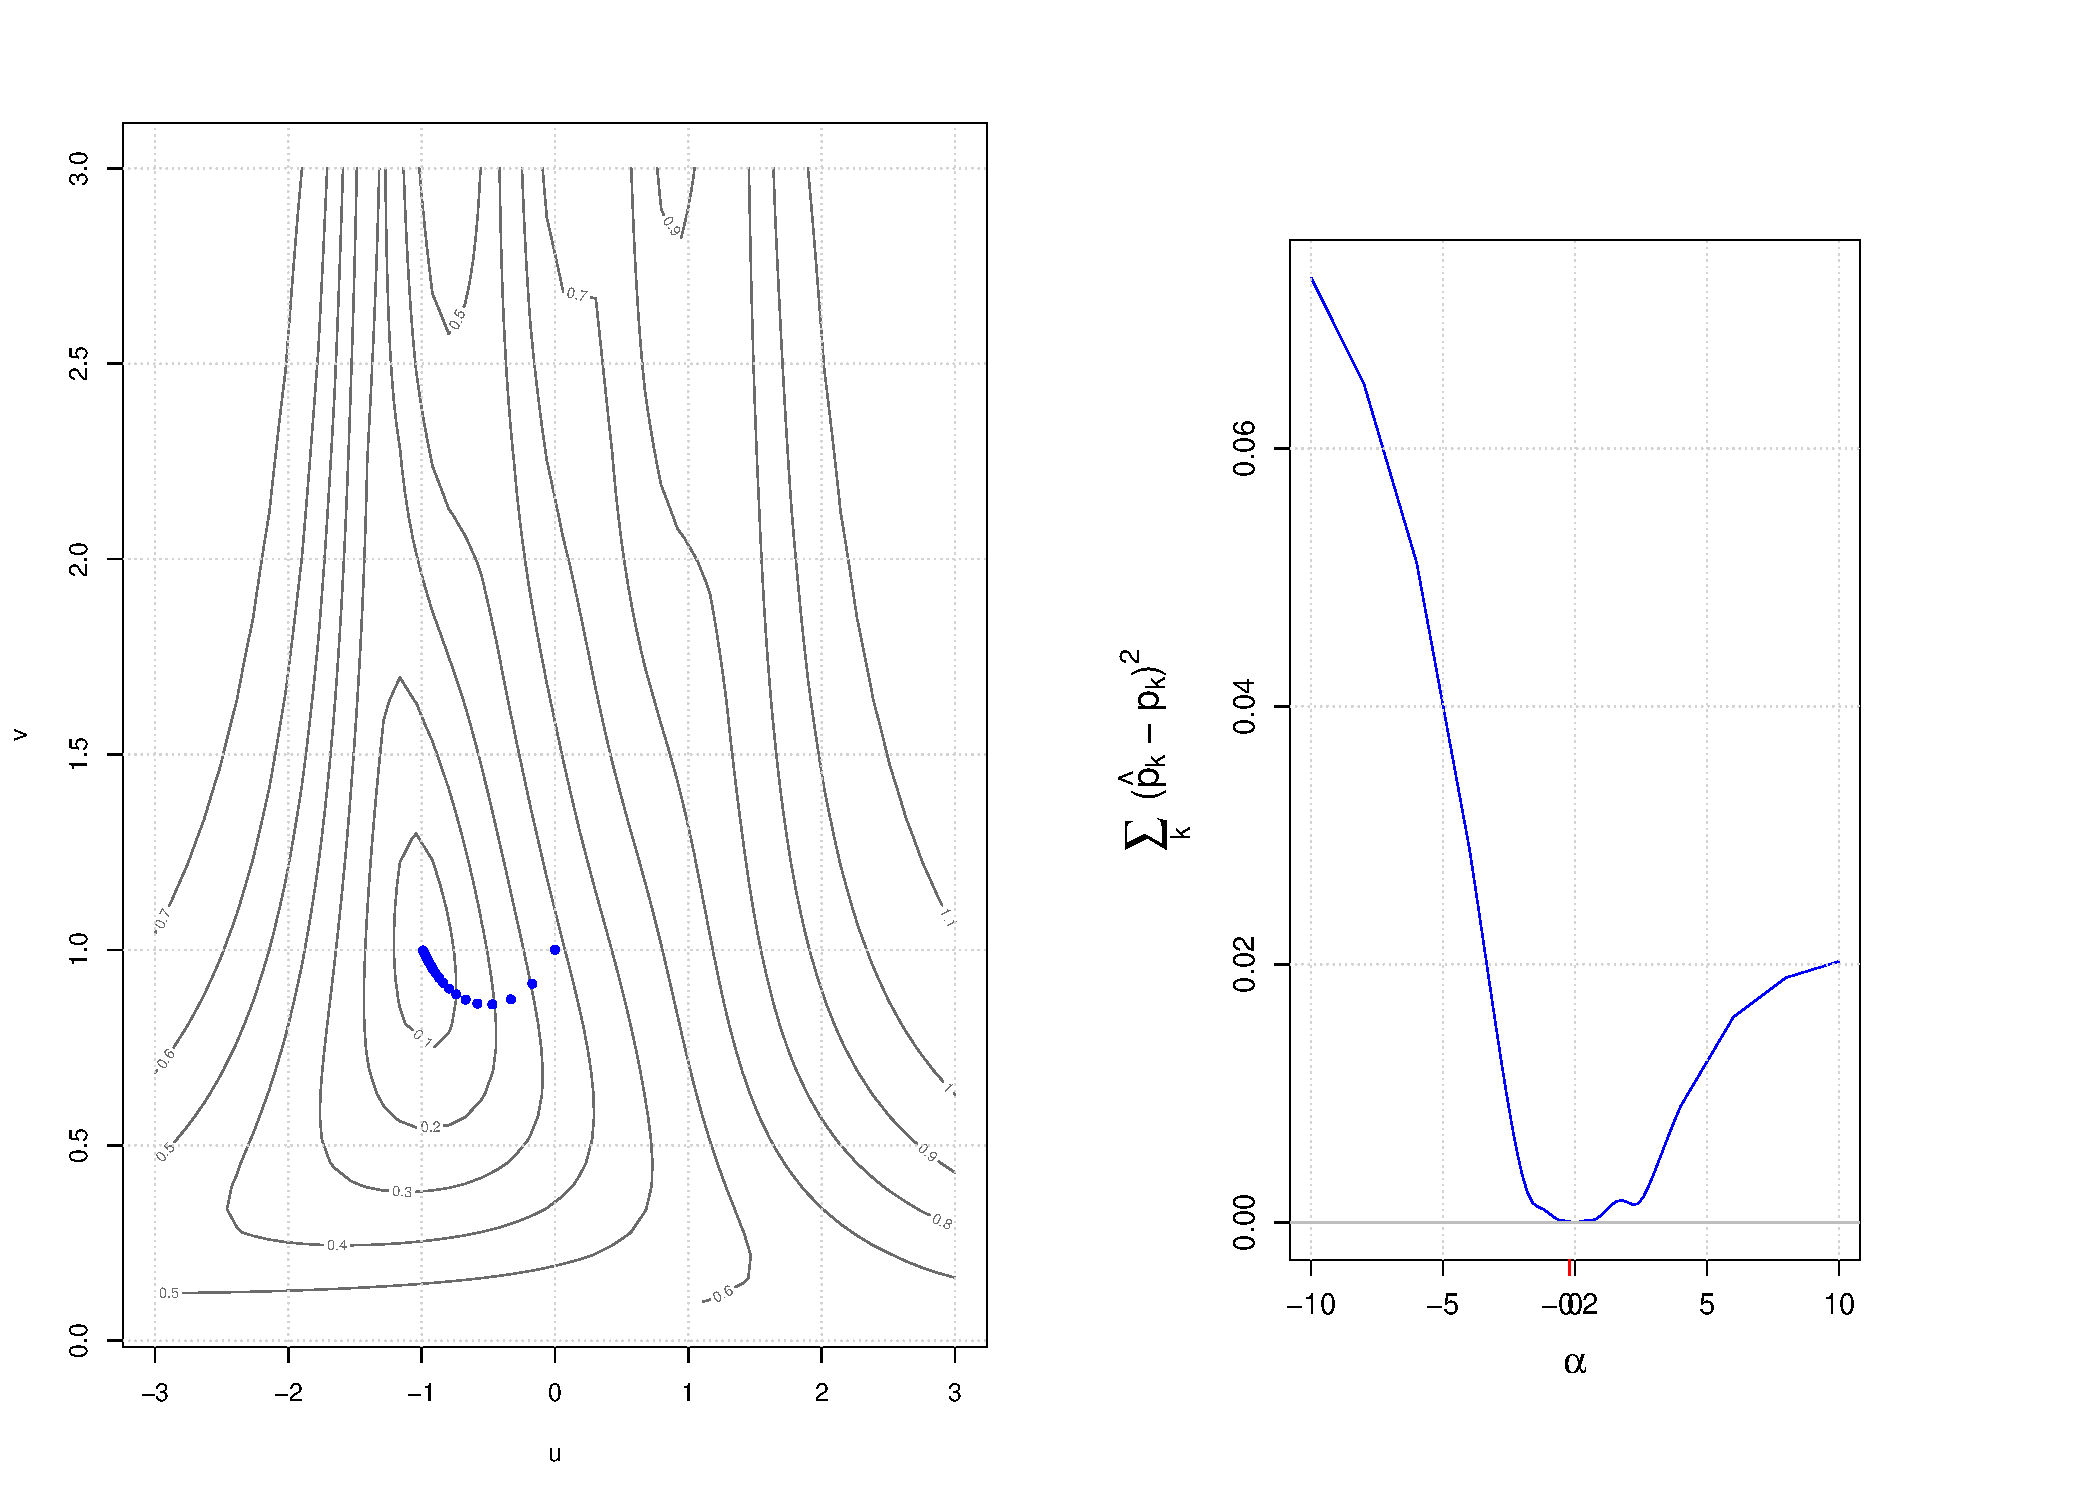
\includegraphics[width=0.8\textwidth]{alpha_0_trace_close_is_good_enough.pdf}
\caption{ Reconstruction from a sample.}
\label{fig: reconstruction_on_sample}
\end{figure}



\section{Comparison of two means} \label{sec: comparison-problem}
Say we use a survey and gather the answers of a random sample of people to questions by which we measure agreement with some abstract idea. For example, we measure agreement with non-compliance with rules with a question: ``How much do you agree with: To request state aid for something which you are not entitled'' with 5 possible responses: completely disagree, ..., completely agree. And say we only want to find out if there is a difference between the mean values of agreement between two populations, for example between male and female populations. We would like to reject the null hypothesis that there is no difference and conclude, for example, that men on average agree more with non-compliance than women.

In this context, a nonparametric test Mann-Whitney is often proposed~\cite{Winter}, however this tests different null hypothesis, namely whether the samples are coming from populations with same distribution. We can also try to use a model for analyzing ordinal data, the so-called proportional odds model, and then test the influence of dichotomous covariant variable (e.g. gender) on the ordinal response~\cite{McCullagh}. However, we obtain the same test statistic as with the Mann-Whitney test, proof in~\cite{Natarajan}. We can also compare the response rates between the groups with $\chi^{2}$-square test. If we only want to find out if there is a difference between the mean values, this tests are not suitable. One of the most commonly used approach is to apply t-test on encoded responses directly.

\subsection{Common testing procedure} \label{sec: fail_test_stat}
The sum of responses $r_{k}$ is not defined in general. For example: completely disagree + ... + completely agree = ? Therefore the common practice is to first {\it encode} the responses. This means to map the responses to some set of numbers. In the case of $K$ possible responses, usually into the first $K$ natural numbers, e.g.: completely disagree $\mapsto 1$, ..., completely agree $\mapsto K$. 

Let $r_{k}$ represent encoded responses:
\begin{equation}
r_{k} \in \mathbb{R}, \qquad k = 1,...,K
\end{equation}
and let $\hat{X}$  $k = 1,..., K$ be a manifest variable defined on the encoded responses. Denote the expected value of $\hat{X}$: 
$$
\mathrm{E}[\hat{X}] = \hat{\mu}
$$ and standard deviation:
$$
\mathrm{sd}(\hat{X}) = \hat{\sigma}.
$$
Denote by $\hat{X}_{i, j}$ the response of the individual $i$ to question $j$. Responses $\lbrace \hat{X}_{i, j} \rbrace$ for sample size $n$ from some population to $m$ questions can be represented by table:
\begin{center}
\begin{tabular}{l|rrr}
     & $1 \quad$ & ... & $m \quad$ \\ 
  \hline
  1 & $\hat{X}_{1,1}$ & ... & $\hat{X}_{1,m}$ \rule{0pt}{3ex} \\
  $.$ &  $. \quad$ & & $. \quad$ \rule{0pt}{0.05ex} \\
  $.$ &  $. \quad$ & & $. \quad$ \rule{0pt}{0.05ex} \\
  $.$ &  $. \quad$ & & $. \quad$ \rule{0pt}{0.05ex} \\
  n & $\hat{X}_{n,1}$ & ... & $\hat{X}_{n,m}$ \rule{0pt}{3ex} \end{tabular}
\end{center}

Common practice is to compute the averages of encoded responses by individuals. Denote this average by $\hat{X}_{i}$:
\begin{equation}
\hat{X}_{i} = \frac{1}{m} \sum_{j = 1}^{m} \hat{X}_{i, j}.
\end{equation}

It holds:
\begin{equation}
\mathrm{E}[\frac{1}{n} \sum_{i=1}^{n} \hat{X}_{i}] = \frac{1}{n \cdot m} \sum	_{i=1}^{n} \sum_{j=1}^{m} \hat{X}_{i,j} = \hat{\mu}
\end{equation}

and
\begin{align*}
\mathrm{var}(\hat{X}_{i}) &= \mathrm{var} \left( \frac{1}{m} \sum_{j=1}^{m} \hat{X}_{i, j} \right) \\
&= \frac{1}{m^{2}} \left( \sum_{j=1}^{m} \mathrm{var}(\hat{X}_{i,j}) + \sum_{j_{1} \neq j_{2}} \mathrm{cov}(X_{i,j_{1}}, X_{i, j_{2}})
\right)
\end{align*}

In general, we should model responses to different questions with different latent variables and covariances between pairs of these latent variables. We simplify by accepting the generally accepted assumption~\cite{Alphen} that these questions are equivalent instruments for measuring, e.g. agreement with some abstract idea. Therefore, for each pair $j_{1}, j_{2}$, the following holds:
\begin{equation}
\mathrm{cov}(\hat{X}_{i,j_{1}}, \hat{X}_{i, j_{2}}) = \mathrm{var}(\hat{X}_{i, j})
\end{equation}

and $\mathrm{var}(\hat{X}_{i})$ simplifies to:
\begin{align*}
\mathrm{var}(\hat{X}_{i}) &= \frac{1}{m^{2}} \left( \sum_{j=1}^{m} \mathrm{var}(\hat{X}_{i,j}) + \sum_{j_{1} \neq j_{2}} \mathrm{var}(\hat{X}_{i,j}) 
\right) \\
&= \frac{1}{m^{2}} \left(m \cdot \hat{\sigma}^{2} + m \cdot (m-1)\cdot \hat{\sigma}^{2} \right) \\
&= \hat{\sigma}^{2}.
\end{align*}

Let $\hat{X}_{1}$ and $\hat{X}_{2}$ be two manifest variables defined on encoded responses of two different populations to the same questions. Denote the expected values $\hat{\mu}_{1}$, $\hat{\mu}_{2}$ and standard deviations $\hat{\sigma}_{1}$, $\hat{\sigma}_{2}$ of the manifest variables $\hat{X}_{1}$, $\hat{X}_{2}$ respectively. 

Common practice is to take random samples from manifest variable $\hat{X}_{i}$ of size $n_{i}$, estimate the expected value $\hat{\mu}_{i}$ and standard deviation $\hat{\sigma}_{i}$, for $i = 1, 2$. Then to use for example Welch t-test and estimate the ratio:
\begin{equation}
\frac{\hat{\mu}_{1} - \hat{\mu}_{2}}{
\sqrt{\frac{\hat{\sigma}^{2}_{1}}{n_{1}} + \frac{\hat{\sigma}^{2}_{2}}{n_{2}}}
}
\end{equation}
and finally calculate the $p$-value from $t$-distribution, where the degrees of freedom can be calculated using Satterhaite-Welch correction.

This procedure is a serious simplification because the value of the ratio $\sigma_{1}^{2} / \sigma_{1}^{2}$ is unknown. We must instead use a bit more complicated test statistic for which the distribution is not known in closed-form. By using the likelihood ratio test we also obtain equations that do not have a closed-form solution and must use an algorithm to solve them.


\subsection{Problem with the common testing procedure}

We show that the common testing procedure is not suitable for mean comparison when variances of latent variables differ. It is not suitable even in the best case when we assume optimal discretization. We also show this problem persist if we use the bootstrap test or permutation test this time only by a simulation study at the end.

Let's look at a simple example where we obtain biased test statistics using the common testing procedure. Pairs of latent and manifest variables for this example are shown in Figure~\ref{fig: problem-definition}.

Imagine again a neutral population with standard normal latent variable $X_{0} \sim N(0,1)$ and suppose the corresponding manifest variable is optimal discretization $\hat{X_{0}}$ of $X_{0}$ with thresholds $x_{k}$ and representatives $r_{k}$ for $k = 1, ..., K$.

Now suppose we have a population with latent variable $X_{1} \sim X_{0} - 1$, we can imagine that, on average, they agree less with this abstract idea then the neutral population. And suppose we have another population with latent variable $X_{2} \sim 0.5 \cdot X_{0} - 1$, we can imagine that, on average, they agree the same as the second population, but their agreement is less dispersed.

It holds:
\begin{equation}
\mathrm{E}[X_{1}] - \mathrm{E}[X_{2}] = 0
\end{equation}
but
\begin{equation}
\mathrm{E}[\hat{X}_{1}] - \mathrm{E}[\hat{X}_{2}] \approx 0.13.
\end{equation}
In this case, we used optimal discretization. The difference is of course not equal to 0 if we use the EW discretization.

\begin{prop}
The test statistic in common testing procedure is biased in general.
\end{prop}
\begin{proof}
Let there be two populations with latent variables $X_{1}$, $X_{2}$ and corresponding manifest variables $\hat{X_{1}}$, $\hat{X_{2}}$. Assume that to both populations are available the same responses on the questionnaire. Assume the representatives $r_{k}$, on which manifest variables are defined, are real numbers or encoded responses from the questionnaire. Then 

\begin{equation}
\mathrm{E}[\hat{X_{i}}] = \mathrm{E}[X_{i}] + \delta_{i}
\end{equation}
for some $\delta_{i} \in \mathcal{R}$ and

\begin{equation}
\mathrm{var}(\hat{X}_{i}) = \mathrm{var}(X_{i}) + \epsilon_{i}
\end{equation}
for positive real number $\epsilon_{i}$ that depends on $X_{i}$ for $i = 1,2$.

With the common procedure, based on sample from manifest variable of size $n_{i}$, we estimate the test statistic:
\begin{align}
T &= \frac{
\mathrm{E}[\hat{X}_{1}] - \mathrm{E}[\hat{X}_{2}]
}{
\sqrt{
\frac{\mathrm{var}(\hat{X}_{1})}{n_{1}} + 
\frac{\mathrm{var}(\hat{X}_{2})}{n_{2}}
}
} \\
&= \frac{
\mathrm{E}[X_{1}] + \delta_{1} - \mathrm{E}[X_{2}] - \delta_{2}
}{
\sqrt{
\frac{\mathrm{var}(X_{1}) + \epsilon_{1} }{n_{1}} + 
\frac{\mathrm{var}(X_{2}) + \epsilon_{2} }{n_{2}}
}
}
\end{align}

Now suppose that:
\begin{equation}
\mathrm{var}(X_{1}) \neq \mathrm{var}(X_{2})
\end{equation}

and:
\begin{equation}
\mathrm{E}[X_{1}] = \mathrm{E}[X_{2}].
\end{equation}

The same answers on the questionnaire are available to both populations. Threrefore, the manifest variables $\hat{X}_{1}$, $\hat{X}_{2}$ are defined on the same domain $r_{k}$, $k = 1,...,K$. Then $\hat{X}_{1}$ and $\hat{X}_{2}$ cannot be both optimal discretizations of latent variables $X_{1}$ and $X_{2}$. Therefore, $\delta_{1}$ and $\delta_{2}$ cannot both be zero. So the difference $\mathrm{E}[\hat{X}_{1}] - \mathrm{E}[\hat{X}_{2}]$ can be arbitrarily large. 
\end{proof}


\subsection{Proposed testing procedure on a concrete example} \label{sec: example}
We illustrate our proposed testing procedure and common testing procedure on a concrete example. Data is from the World Values Survey from Sweden in 2011~\cite{WVS}. The responses are values from 1 to 10. A value of 1 means the least agreement and a value of 10 the most agreement with how justifiable the claim is. The surveyed Swedes responded to the following claims:
\begin{itemize}
  \item Claiming government benefits to which you are not entitled.
  \item Avoiding a fare on public transport.
  \item Stealing property.
  \item Cheating on taxes if you have a chance.
  \item Someone accepting a bribe in the course of their duties.
\end{itemize}

We suppose all the questions are equivalent instruments for measuring agreement with some abstract idea in this case the idea can be described as non-compliance with the rules.

We have a sample of $n_{1} = 540$ male responses and a sample of $n_{2} = 584$ female responses to these 5 claims. With common testing procedure we get $p$-value $\approx 0.10341$. 

Let's illustrate our testing procedure for comparing means described in~\ref{sec: reconstruction}. We assume that agreement follows skew-normal distribution and compute estimates for $p_{k}$ of manifest random variable $\hat{X}_{1}$ for male population, by dividing the number of male responses with the number of questions 5: $540 \cdot 5$ and similar for female responses. We obtain estimates of the manifest variables shown in Figure~\ref{fig: estimates}. 

\begin{figure}
\centering
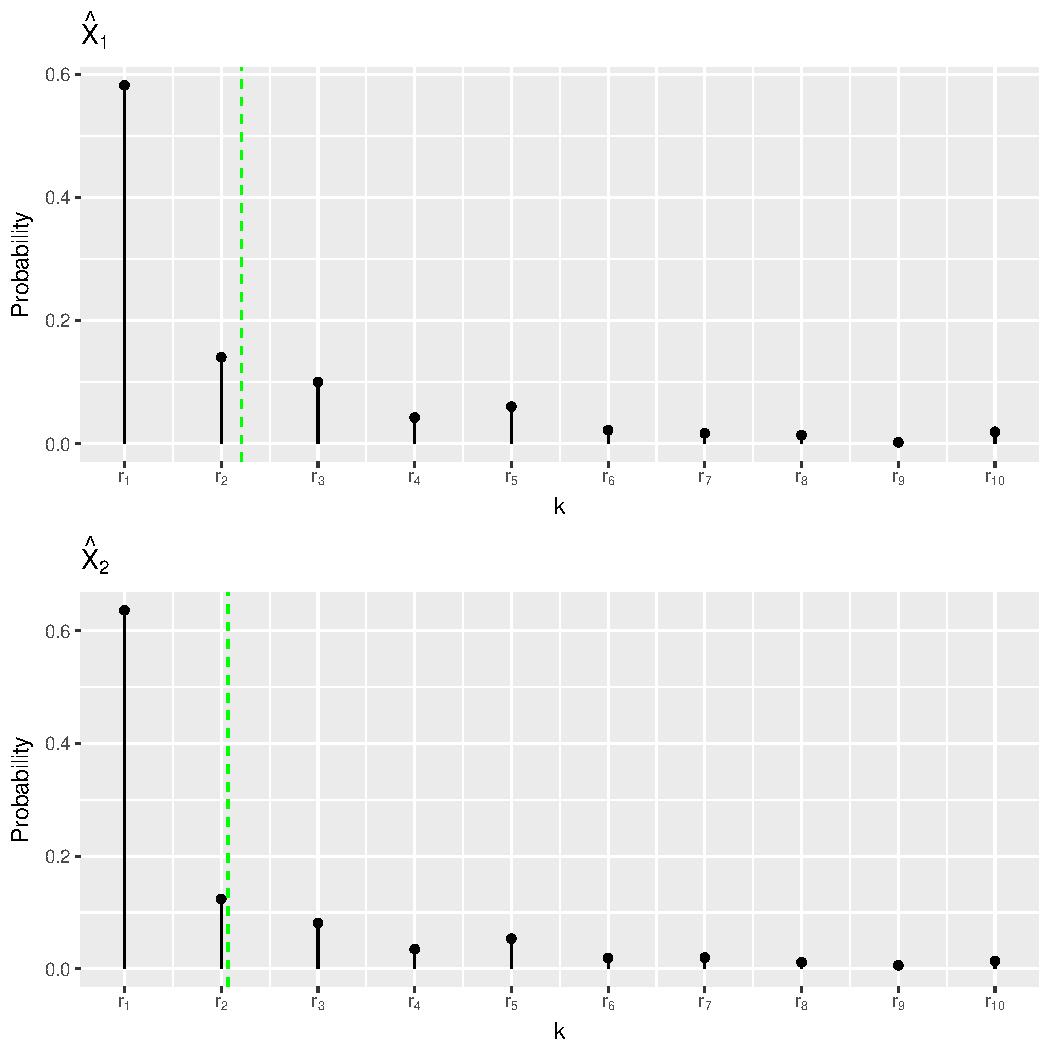
\includegraphics[width=0.6\textwidth]{example.pdf}
\caption{ Estimated manifest variables for male and female populations.}
\label{fig: estimates}
\end{figure}

Let $X_{1}$, $X_{2}$ be latent variables for male and female populations and assume optimal thresholds so we can reconstruct both latent variables. For both populations, we obtain $\alpha_{1} = \alpha_{2} = -1.2$. The trace of the adaptive Gauss-Newton method and the function of error $\epsilon$ in terms of $\alpha$ based on male responses is shown in Figure~\ref{fig: estimates2}. Estimates $\mu_{i}$ and standard deviation $\sigma_{i}$ for $X_{i}$, $i = 1, 2$ is:
\begin{align*}
\hat{\mu}_{1} &= \xi_{1} \approx -3.33, \\
\hat{\sigma}_{1} &= \omega_{1} \cdot \mathrm{sd}(X_{0}) \approx 2.97, \\
\hat{\mu}_{2} &= \xi_{2} \approx -2.99, \\
\hat{\sigma}_{1} &= \omega_{1} \cdot \mathrm{sd}(X_{0}) \approx 3.25,
\end{align*}
where $X_{0} \sim SN(-1.2)$.

Finally we calculate test statistics:
\begin{equation}
t = \frac{\hat{\mu}_{1} - \hat{\mu}_{2}}{
\sqrt{\frac{\hat{\sigma}_{1}}{n_{1}} + \frac{\hat{\sigma}_{2}}{n_{2}}}
}
\end{equation}

and $p$-value from $t$-distribution, where we calculate the degrees of freedom with Satterthaite-Welch correction and obtain $p$-value $\approx 0.06449033$. 

\begin{figure}
\centering
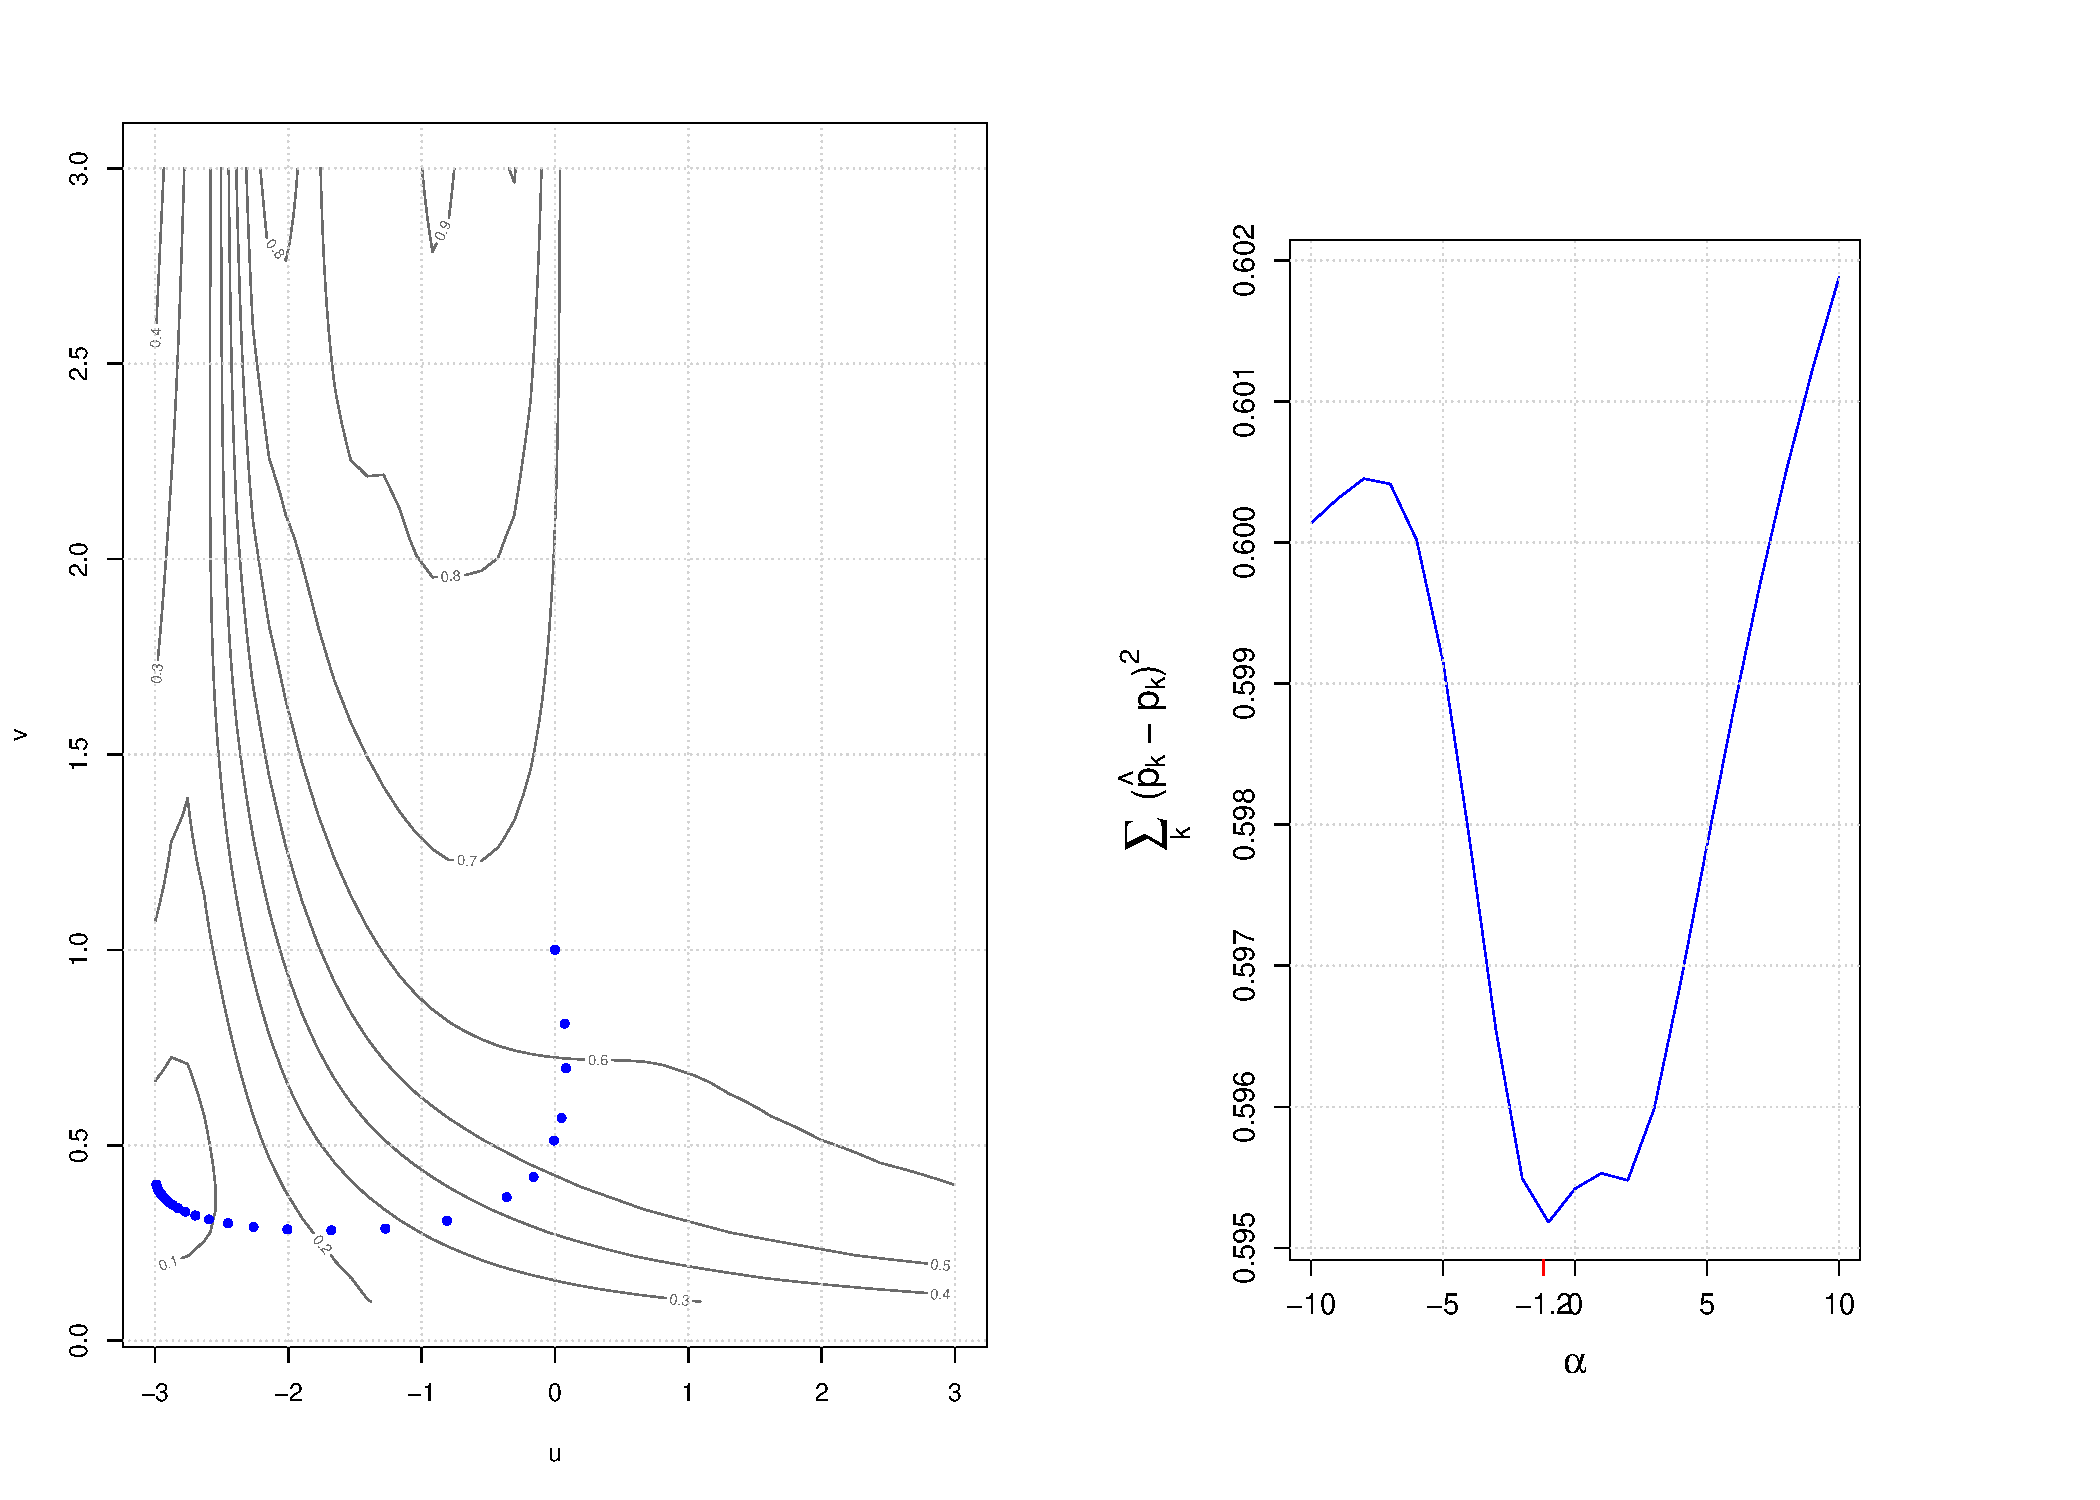
\includegraphics[width=0.8\textwidth]{example_estimation.pdf}
\caption{ Trace of the Gauss-Newton method and function of error $\epsilon$ in terms of $\alpha$ based on male responses.}
\label{fig: estimates2}
\end{figure}

\section{Conclusions}
We introduce a model to explore the relationship between Likert-type responses and underlying hypothetical latent variables. Then derive the optimal relationship in the form of discretization and reconstruction procedures. We use this discretization procedure to simulate Likert-type responses. We then show the problem with the common approach to comparison of two means in the context of our model. And propose an alternative approach where we illustrate the use of our reconstruction procedure. Source code is available at:

\url{https://github.com/markolalovic/latent-variable-reconstruction}

\bibliographystyle{ieeetr}
\bibliography{main}

\end{document}
